\documentclass[handout]{beamer}
\usetheme{Marburg}
\useoutertheme{infolines}
\newcommand{\answers}{1}

\usepackage{amsmath}
\usepackage{caption}
\usepackage{color}
\usepackage{enumerate}
\usepackage{listings}
\usepackage{hyperref}
\usepackage{mathrsfs}
\usepackage{natbib}
\usepackage{url}

\providecommand{\all}{\ \forall \ }
\providecommand{\bs}{\backslash}
\providecommand{\e}{\varepsilon}
\providecommand{\E}{\ \exists \ }
\providecommand{\lm}[2]{\lim_{#1 \rightarrow #2}}
\providecommand{\m}[1]{\mathbb{#1}}
\providecommand{\nv}{{}^{-1}}
\providecommand{\ov}[1]{\overline{#1}}
\providecommand{\p}{\newpage}
\providecommand{\q}{$\quad$ \newline}
\providecommand{\rt}{\rightarrow}
\providecommand{\Rt}{\Rightarrow}
\providecommand{\vc}[1]{\boldsymbol{#1}}
\providecommand{\wh}[1]{\widehat{#1}}

\hypersetup{colorlinks,linkcolor=,urlcolor=blue}
\numberwithin{equation}{section}

\definecolor{dkgreen}{rgb}{0,0.6,0}
\definecolor{gray}{rgb}{0.5,0.5,0.5}
\definecolor{mauve}{rgb}{0.58,0,0.82}

\lstset{ 
  language=C,                % the language of the code
  basicstyle= \footnotesize,           % the size of the fonts that are used for the code
  numbers=left,
  numberfirstline=true,
  numbersep=5pt,                  % how far the line-numbers are from the code
  backgroundcolor=\color{white},      % choose the background color. You must add \usepackage{color}
  showspaces=false,               % show spaces adding particular underscores
  showstringspaces=false,         % underline spaces within strings
  showtabs=false,                 % show tabs within strings adding particular underscores
  frame=lrb,                   % adds a frame around the code
  rulecolor=\color{black},        % if not set, the frame-color may be changed on line-breaks within not-black text 
  tabsize=2,                      % sets default tabsize to 2 spaces
  captionpos=t,                   % sets the caption-position 
  breaklines=true,                % sets automatic line breaking
  breakatwhitespace=false,        % sets if automatic breaks should only happen at whitespace
  %title=\lstname,                   % show the filename of files included with \lstinputlisting;
  keywordstyle=\color{blue},          % keyword style
  commentstyle=\color{gray},       % comment style
  stringstyle=\color{dkgreen},         % string literal style
  escapeinside={\%*}{*)},            % if you want to add LaTeX within your code
  morekeywords={*, ...},               % if you want to add more keywords to the set
  xleftmargin=0.2in, % left horizontal offset of caption box
  xrightmargin=-.03in % right horizontal offset of caption box
}

%\DeclareCaptionFont{white}{\color{white}}
%\DeclareCaptionFormat{listing}{\parbox{\textwidth}{\colorbox{gray}{\parbox{\textwidth}{#1#2#3}}\vskip-0.05in}}
%\captionsetup[lstlisting]{format = listing, labelfont = white, textfont = white}
%For caption-free listings, comment out the 3 lines above and uncomment the 2 lines below.
 \captionsetup{labelformat = empty, labelsep = none}
 \lstset{frame = single}

\title{The CURAND library}
\author{Will Landau}
\date{November 4, 2013}
\institute{Iowa State University}

\begin{document}

\begin{frame}
\titlepage
 \end{frame}
 
 \begin{frame}
\frametitle{Outline}
\tableofcontents
\end{frame}
 
 \AtBeginSection[]
{
   \begin{frame}
       \frametitle{Outline}
       \tableofcontents[currentsection]
   \end{frame}
}


\begin{frame}
\frametitle{CURAND}
\begin{itemize}
\item {\bf CURAND}: a CUDA C library for quickly generating pseudorandom and quasi-random numbers.
\pause \item {\bf Pseudorandom sequence}: a sequence of numbers, generated by a deterministic algorithm, that has most of the properties of a truly random sequence.
\pause \item {\bf Quasi-random (low-discrepancy) sequence}: a sequence of $n$-dimensional points, generated by a deterministic sequence, that appear random and appear to fill a region of $n$-dimensional space evenly.
\end{itemize}
\end{frame}


\begin{frame}
\frametitle{Host and device APIs}
\begin{itemize}
\item Host API
\begin{itemize}
\pause \item Include the header, {\tt curand.h}, and link with the {\tt -lcurand} flag at compilation. 
\pause \item Calls to number generators happen on the host.
\pause \item With each call, a predetermined number of random draws is generated and then stored for alter use in a kernel call or a copy statement.
\pause \item Supports 3 pseudorandom generators and 4 quasi-random generators.
\end{itemize}
\pause \item Device API
\begin{itemize}
\pause \item Include the header, {\tt curand\_kernel.h}, and link with the {\tt -lcurand} flag at compilation.
\pause \item Calls to number generators happen within kernels and device functions.
\pause \item Random numbers are generated and immediately used in real time on an as-need basis.
\pause \item For CUDA version 4.2, supports fewer generator algorithms then the host API.
\end{itemize}
\end{itemize}
\end{frame}

\section{Host interface}

\begin{frame}
\frametitle{Using the host API}
\begin{enumerate}
\pause \item Create a new generator with {\tt curandCreateGenerator()}.
\pause \item Set the generator options. For example, use {\tt curandSetPseudoRandomGeneratorSeed()} to set the seed.
\pause \item Allocate memory for the random numbers with {\tt cudaMalloc()}.
\pause \item Generate random numbers with on or more calls to {\tt curandGenerate()} or another generation function.
\pause \item Clean up the generator with {\tt curandDestroyGenerator()}.
\pause \item Clean up everything else with {\tt free()} and {\tt cudaFree()}.
\end{enumerate}
\end{frame}

\begin{frame}
\frametitle{Generator types for {\tt curandCreateGenerator()}}
\begin{itemize}
\item Pseudorandom number generators
\begin{itemize}
\pause \item {\tt CURAND\_RNG\_PSEUDO\_DEFAULT}: XORWOW for the version currently on impact1
\pause \item {\tt CURAND\_RNG\_PSEUDO\_XORWOW}: XORWOW algorithm
\pause \item {\tt CURAND\_RNG\_PSEUDO\_MRG32K3A}: combined multiple recursive family
\pause \item {\tt CURAND\_RNG\_PSEUDO\_MTGP32}: Mersenne Twister family
\end{itemize}
\pause \item Quasi-random number generators
\begin{itemize}
\pause \item {\tt CURAND\_RNG\_QUASI\_DEFAULT}: currently Sobol, 32-bit sequences
\pause \item {\tt CURAND\_RNG\_QUASI\_SOBOL32}: Sobol, 32-bit sequences
 \item {\tt CURAND\_RNG\_QUASI\_SOBOL64}: Sobol, 62-bit sequences
\pause \item {\tt CURAND\_RNG\_QUASI\_SCRAMBLED\_SOBOL32}: scrambled Sobol, 32-bit sequences
 \item {\tt CURAND\_RNG\_QUASI\_SCRAMBLED\_SOBOL64}: scrambled Sobol, 62-bit sequences
\end{itemize}
\end{itemize}
\end{frame}

\begin{frame}
\frametitle{Generator options}
\begin{itemize}
\item {\bf Seed}: a 64-bit integer that initializes the starting state of a pseudorandom number generator.
\pause \item {\bf Offset}: a parameter used sot skip ahead in the sequence. Set offset = 100 to return the 100th number in the sequence first. Not available for the Mersenne Twister.
\pause \item {\bf Order}: a parameter specifying how results are ordered in global memory.
\end{itemize}
\end{frame}

\begin{frame}[fragile]
\frametitle{Generator functions}
\begin{itemize}
\item Random bits:
\lstset{basicstyle=\tiny}
\begin{lstlisting}
curandStatus_t curandGenerate(curandGenerator_t generator, unsigned int *outputPtr, size_t num)
\end{lstlisting}

\pause \item Uniform(0, 1):
\begin{lstlisting}
curandStatus_t curandGenerateUniform(curandGenerator_t generator, float *outputPtr, size_t num)

curandStatus_t curandGenerateUniformDouble(curandGenerator_t generator, double *outputPtr, size_t num)
\end{lstlisting}

\pause \item Normal:
\begin{lstlisting}
curandStatus_t curandGenerateNormal(curandGenerator_t generator, float *outputPtr, size_t n, float mean, float stddev)

curandStatus_t curandGenerateNormalDouble(curandGenerator_t generator, double *outputPtr, size_t n, double mean, double stddev)
\end{lstlisting}
\end{itemize}
\end{frame}


\begin{frame}[fragile]
\frametitle{Generator functions} \lstset{basicstyle=\tiny}
\begin{itemize}

\item Log-normal:
\begin{lstlisting}
curandStatus_t curandGenerateLogNormal(curandGenerator_t generator, float *outputPtr, size_t n, float mean, float stddev)

curandStatus_t curandGenerateLogNormalDouble(curandGenerator_t generator, double *outputPtr, size_t n, double mean, double stddev)
\end{lstlisting}
\end{itemize}
\end{frame}


\begin{frame}[fragile]
\frametitle{Example: {\tt host\_api.cu}} \lstset{basicstyle=\tiny}
\begin{lstlisting}[name=host]
/*
* This program uses the host CURAND API to generate 10 pseudorandom floats.
*/

#include <stdio.h> 
#include <stdlib.h>
#include <cuda.h> 
#include <curand.h>

int main(int argc, char *argv[]){
  size_t n = 10;
  size_t i; 
  curandGenerator_t gen; 
  float *devData , *hostData;

 /* Allocate n floats on host */
  hostData = (float *) calloc(n, sizeof(float));
  
  /* Allocate n floats on device */ 
  cudaMalloc((void **) &devData, n*sizeof(float));

  /* Create a Mersenne Twister pseudorandom number generator */ 
  curandCreateGenerator(&gen, CURAND_RNG_PSEUDO_MTGP32);

  /* Set seed */ 
  curandSetPseudoRandomGeneratorSeed(gen, 1234ULL);
  
  /* Generate n floats on device */
  curandGenerateUniform(gen, devData, n);

\end{lstlisting}
\end{frame}

\begin{frame}[fragile]
\frametitle{Example: {\tt host\_api.cu}} \lstset{basicstyle=\tiny}
\begin{lstlisting}[name=host]
 /* Copy device memory to host */ 
  cudaMemcpy(hostData , devData , n * sizeof(float), cudaMemcpyDeviceToHost);

  /* Show result */
  printf("Random Unif(0, 1) draws:\n");
  for(i = 0; i < n; i++) {
    printf("  %1.4f\n", hostData[i]); 
  }
  printf("\n");

  /* Cleanup */ 
  curandDestroyGenerator(gen); 
  cudaFree(devData);
  free(hostData);
}
\end{lstlisting}

\pause \begin{lstlisting}
> nvcc host_api.cu -lcurand -o host_api
> ./host_api
Random Unif(0, 1) draws:
  0.5823
  0.4636
  0.6156
  0.9964
  0.1182
  0.2672
  0.9241
  0.7161
  0.2309
  0.4075
\end{lstlisting}
\end{frame}







\section{Device interface}


\begin{frame}
\frametitle{Using the Device API}
\begin{enumerate}
\item Within a kernel, call {\tt curand\_init()} to initialize the ``state" of the random number generator.
\pause \item Within a (possibly separate) kernel, call {\tt curand()} or one of its wrapper functions (such as {\tt curand\_uniform()} or {\tt curand\_normal()} to generate pseudorandom or quasi random numbers as needed.
\end{enumerate}

\begin{itemize}
\pause \item RNG types available
\begin{itemize}
\pause \item Pseudorandom
\begin{itemize}
\item XORWOW
\end{itemize}
\pause \item Quasi-random
\begin{itemize}
\item 32-bit Sobol
\item 32-bit scrambled Sobol
\end{itemize}
\end{itemize}
\end{itemize}
\end{frame}


\begin{frame}[fragile]
\frametitle{Device API functions: XORWOW}

\lstset{basicstyle=\tiny}
\begin{lstlisting}
__device__ void curand_init (unsigned long long seed, 
                             unsigned long long sequence,
                             unsigned long long offset, 
                             curandState_t *state)

__device__ unsigned int 
curand (curandState_t *state) // RANDOM BITS

__device__ float
curand_uniform (curandState_t *state) // U(0,1)

__device__ double
curand_uniform_double (curandState_t *state) // U(0,1)

__device__ float
curand_normal (curandState_t *state) // N(0,1)

__device__ double
curand_normal_double (curandState_t *state) // N(0,1)
\end{lstlisting}
\end{frame}

\begin{frame}[fragile]
\frametitle{Device API functions: XORWOW}
\lstset{basicstyle=\tiny}
\begin{lstlisting}
__device__ float2
curand_normal2 (curandState_t *state) // 2 N(0,1) draws

__device__ float2
curand_log_normal2 (curandState_t *state) // 2 N(0,1) draws

__device__ float
curand_log_normal (curandState_t *state, float mean, float stddev)

__device__ double
curand_log_normal_double (curandState_t *state, double mean, double stddev)

__device__ double2
curand_normal2_double (curandState_t *state) // 2 draws

__device__ double2
curand_log_normal2_double (curandState_t *state) // 2 draws
\end{lstlisting}
\end{frame}






\begin{frame}[fragile]
\frametitle{Device API functions: Sobol}

\lstset{basicstyle=\tiny}
\begin{lstlisting}
__device__ void
curand_init (
    unsigned int *direction_vectors,
    unsigned int offset,
    curandStateSobol32_t *state) // Sobol 

__device__ void
curand_init (
    unsigned int *direction_vectors,
    unsigned int scramble_c,
    unsigned int offset,
    curandStateScrambledSobol32_t *state) // Scrambled Sobol
    
__device__ unsigned int
curand (curandStateSobol32_t *state)

__device__ float
curand_uniform (curandStateSobol32_t *state)
\end{lstlisting}
\end{frame}

\begin{frame}[fragile]
\frametitle{Device API functions: Sobol}
\lstset{basicstyle=\tiny}
\begin{lstlisting}
__device__ float
curand_normal (curandStateSobol32_t *state)

__device__ float
curand_log_normal (
    curandStateSobol32_t *state,
    float mean,
    float stddev)

__device__ double
curand_uniform_double (curandStateSobol32_t *state)

__device__ double
curand_normal_double (curandStateSobol32_t *state)

__device__ double
curand_log_normal_double (
    curandStateSobol32_t *state,
    double mean,
    double stddev)

\end{lstlisting}
\end{frame}






\begin{frame}[fragile]
\frametitle{Example: {\tt device\_api.cu}} \lstset{basicstyle=\tiny}
\begin{lstlisting}[name=dev]
/*
 * This program uses the device CURAND API to calculate what 
 * proportion of pseudo-random ints are odd.
 */

#include <stdio.h>
#include <stdlib.h> 
#include <cuda.h>
#include <curand_kernel.h>

__global__ void setup_kernel(curandState *state){
  int id = threadIdx.x + blockIdx.x * 64;

  /* Each thread gets same seed, a different sequence number , no offset */
  curand_init(1234, id, 0, &state[id]); 
}

__global__ void generate_kernel(curandState *state, int *result){
  int id = threadIdx.x + blockIdx.x * 64; int count = 0;
  unsigned int x;

  /* Copy state to local memory for efficiency */ 
  curandState localState = state[id];
  
  /* Generate pseudo -random unsigned ints */ 
  for(int n = 0; n < 100000; n++){
    x = curand(&localState); 
\end{lstlisting}
\end{frame}


\begin{frame}[fragile]
\frametitle{Example: {\tt device\_api.cu}} \lstset{basicstyle=\tiny}
\begin{lstlisting}[name=dev]
    /* Check if odd */ 
    if(x & 1){
      count ++; 
    }
  }

  /* Copy state back to global memory */ 
  state[id] = localState;

  /* Store results */
  result[id] += count;
}

int main(int argc, char *argv[]){
  int i, total;

  int *devResults, *hostResults;
  curandState *devStates;

  /* Allocate space for results on host */ 
  hostResults = (int *) calloc(64 * 64, sizeof(int));
  
  /* Allocate space for results on device */ 
  cudaMalloc((void **)&devResults , 64 * 64 *sizeof(int));
  
  /* Set results to 0 */ 
  cudaMemset(devResults , 0, 64 * 64 * sizeof(int));
  
  /* Allocate space for prng states on device */ 
  cudaMalloc((void **)&devStates , 64 * 64 * sizeof(curandState)); 
 
\end{lstlisting}
\end{frame}


\begin{frame}[fragile]
\frametitle{Example: {\tt device\_api.cu}} \lstset{basicstyle=\tiny}
\begin{lstlisting}[name=dev]
  /* Setup prng states */
  setup_kernel<<<64, 64>>>(devStates);

  /* Generate and use pseudorandom numbers*/ 
  for(i = 0; i < 10; i++){
    generate_kernel<<<64, 64>>>(devStates, devResults);
  }
  
  /* Copy device memory to host */ 
  cudaMemcpy(hostResults, devResults , 64 * 64 * sizeof(int), cudaMemcpyDeviceToHost);

  /* Show result */
  total = 0;
  for(i = 0; i < 64 * 64; i++) {
    total += hostResults[i];
  }
  printf("Fraction odd was %10.13f\n", (float) total / (64.0f * 64.0f * 100000.0f * 10.0f)); 

  /* Cleanup */
  cudaFree(devStates);
  cudaFree(devResults);
  free(hostResults);
  
  return EXIT_SUCCESS;
}
\end{lstlisting}
\end{frame}


\begin{frame}[fragile]
\frametitle{Example: {\tt device\_api.cu}} \lstset{basicstyle=\tiny}
\lstset{language=bash}
\begin{lstlisting}
> nvcc device_api.cu -lcurand -o device_api
ptxas /tmp/tmpxft_000020d0_00000000-2_device_api.pts, line 501;
  warning : Double is not supported. Demoting to float.
>
> ./device_api
Fraction odd was 0.4999966323376
\end{lstlisting}
\end{frame}



\section{Rejection sampling on the GPU}


\begin{frame}
\frametitle{RNG types supported}
\begin{itemize}
\item Dr. Jarad Niemi wrote example rejection sampling code available at \url{https://github.com/jarad/gpuRejectionSampling}.
\pause \item Idea
\begin{enumerate}
 \item Draw a pseudorandom number, $x$.
\pause \item If $x$ is too big, throw out $x$ and return to step 1.
\pause \item Return $x$.
\end{enumerate}
\end{itemize}
\end{frame}



\begin{frame}[fragile]
\frametitle{{\tt cpu\_runif.c}} \lstset{basicstyle=\tiny}
\begin{lstlisting}[name=cpurunif]
#include <Rmath.h>
//#include <stdlib.h>


int cpu_runif(int n, double ub, int ni, int nd, double *u, int *count)
{
    int i, j, a;
    double b;
    GetRNGstate();
    for (i=0;i<n;i++) {
        count[i] = -1;
        u[i] = ub+1;

        while ( u[i]>ub  ) {
            count[i]++;
            //u[i] = rand()/((double)RAND_MAX + 1);
            u[i] = runif(0,1);

            // Computational overhead
            a=0; for (j=0; j<ni; j++) a += 1;
            b=1; for (j=0; j<nd; j++) b *= 1.00001;
        }
    }
    PutRNGstate();
}

void cpu_runif_wrap(int *n, double *ub, int *ni, int *nd, double *u, int *count){
    cpu_runif(*n, *ub, *ni, *nd, u, count);
}
\end{lstlisting}
\end{frame}





\begin{frame}[fragile]
\frametitle{{\tt gpu\_runif.cu}} \lstset{basicstyle=\tiny}
\begin{lstlisting}[name=gpurunif]
#include <curand_kernel.h>
#include "cutil_inline.h"

#define THREADS_PER_BLOCK 256

__global__ void setup_prng(unsigned long long seed, curandState *state)
{
    int id = threadIdx.x + blockIdx.x * THREADS_PER_BLOCK;
    curand_init(seed, id, 0, &state[id]);
}

__global__ void runif_kernel(curandState *state, double ub, int ni, int nd, 
                             double *uniforms, int *counts)
{
    int i, a, count, id = threadIdx.x + blockIdx.x * THREADS_PER_BLOCK;
    double b, u;

    // Copy state to local memory for efficiency */
    curandState localState = state[id];

    // Find random uniform below the upper bound 
    count  = -1;
    u = ub+1;
\end{lstlisting}
\end{frame}


\begin{frame}[fragile]
\frametitle{{\tt gpu\_runif.cu}} \lstset{basicstyle=\tiny}
\begin{lstlisting}[name=gpurunif]
 while ( u>ub ) 
    {
        count++;
        u = curand_uniform_double(&localState);

        // Computational overhead
        a=0; for (i=0; i<ni; i++) a += 1; 
        b=1; for (i=0; i<nd; i++) b *= 1.00001;
    }

    // Copy state back to global memory */
    state[id] = localState ;

    // Store results */
    uniforms[id] = u;
    counts[id] = count;
}

//CURAND_RNG_PSEUDO_MTGP32

extern "C" {

void gpu_runif(int *n, double *ub, int *ni, int *nd, double *seed, double *u, int *c) 
{
    int nBlocks = *n/THREADS_PER_BLOCK, *d_c;
    size_t u_size = *n *sizeof(double), c_size = *n *sizeof(int);
    double *d_u;

    cutilSafeCall( cudaMalloc((void**)&d_u,  u_size) );
    cutilSafeCall( cudaMalloc((void**)&d_c,  c_size) );
\end{lstlisting}
\end{frame}


\begin{frame}[fragile]
\frametitle{{\tt gpu\_runif.cu}}  \lstset{basicstyle=\tiny}
\begin{lstlisting}[name=gpurunif]
    // Setup prng states
    curandState *d_states;
    cutilSafeCall( cudaMalloc((void**)&d_states, nBlocks*THREADS_PER_BLOCK*sizeof(curandState)) );
    setup_prng<<<nBlocks,THREADS_PER_BLOCK>>>(*seed, d_states);

    runif_kernel<<<nBlocks,THREADS_PER_BLOCK>>>(d_states, *ub, *ni, *nd, d_u, d_c);
 
    cutilSafeCall( cudaMemcpy(u,   d_u,  u_size, cudaMemcpyDeviceToHost) );
    cutilSafeCall( cudaMemcpy(c,   d_c,  c_size, cudaMemcpyDeviceToHost) );

    cutilSafeCall( cudaFree(d_u)      );
    cutilSafeCall( cudaFree(d_c)      );
    cutilSafeCall( cudaFree(d_states) );
}

} // end of extern "C"
\end{lstlisting}
\end{frame}


\begin{frame}[fragile]
\frametitle{{\tt my.unif.r}}  \lstset{basicstyle=\tiny}
\lstset{language=R}
\begin{lstlisting}[name=myunifr]
my.runif = function(n, ub, ni=1, nd=1, 
                      engine="R",  seed=1)
{
    engine = pmatch(engine, c("R","C","GPU"))

    switch(engine,
    {
        # R implementation
        u = rep(Inf,n)
        count = rep(0,n)
        set.seed(seed)

        for (i in 1:n) while( (u[i] <- runif(1))>ub ) 
        {
            count[i] = count[i]+1
            a = 0
            b = 1
            for (j in 1:ni) a = a + 1
            for (j in 1:nd) b = b * 1.00001
        }
        return(list(u=u,count=count))
    },
\end{lstlisting}
\end{frame}

\begin{frame}[fragile]
\frametitle{{\tt my.unif.r}}  \lstset{basicstyle=\tiny}
\lstset{language=R}
\begin{lstlisting}[name=myunifr]
   {
        # C implementation
        set.seed(seed)
        out = .C("cpu_runif_wrap", 
                      as.integer(n), 
                      as.double(ub), 
                      as.integer(ni), 
                      as.integer(nd),
                      u=double(n), 
                      count=integer(n))
        return(list(u=out$u,count=out$count))
    },
    {
        # GPU implementation
        out = .C("gpu_runif", as.integer(n), as.double(ub), 
                              as.integer(ni), as.integer(nd),
                              as.double(seed),
                              u=double(n), count=integer(n))
        return(list(u=out$u,count=out$count))
    })
}
\end{lstlisting}
\end{frame}

\begin{frame}[fragile]
\frametitle{Running the example}  \lstset{basicstyle=\tiny}
\begin{itemize}
\item The files, {\tt comparison.r} and {\tt comparison-analysis.r}, compare the performances of the R, C, and GPU rejection samplers.
\end{itemize}

\begin{lstlisting}[language = bash]
> ls
demo  inst  R  README.md  src
> cd src
> make
/usr/local/cuda/bin/nvcc -arch=sm_20  -c -I. -I/usr/local/include -I/usr/local/cuda/include -I/apps/lib64/R/include -I/usr/local/NVIDIA_GPU_Computing_SDK/C/common/inc -Xcompiler -fpic -DRPRINT -DNDEBUG cpu_runif.c -o cpu_runif.o
...

> cd ..
> ls
demo  inst  R  README.md  src
> cd demo
> ls
comparison.R     comparison-analysis.R     segfault.R
> R CMD BATCH comparison.R & # do this using screen: it takes a couple days unless you modify comparison.R
> R CMD BATCH comparison-analysis.R
> ls
comparison-analysis.R     comparison.csv  comparison.Rout  rejection.pdf  segfault.R
comparison-analysis.Rout  comparison.R    comparison.tex   Rplots.pdf     sm.tex
\end{lstlisting}
\end{frame}

\begin{frame}
\frametitle{Performance: ratios of CPU time to GPU time}
\begin{center}
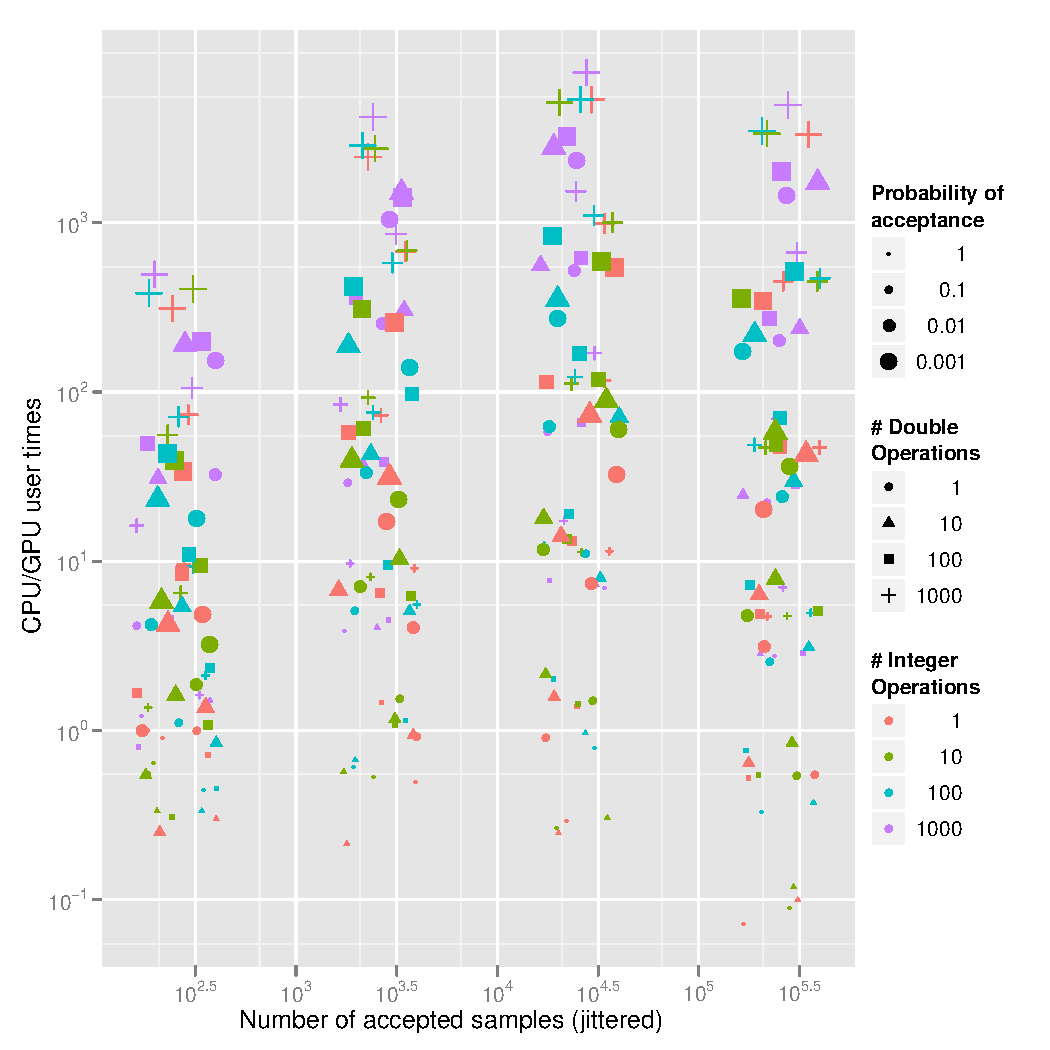
\includegraphics[scale=.42]{../../fig/rejectiontime}
\end{center}
\end{frame}

\begin{frame}
\frametitle{Outline}
\tableofcontents
\end{frame}

\begin{frame}
\frametitle{Resources} \small

\begin{itemize}
\item Guides:
\begin{enumerate}
 \item \href{http://docs.nvidia.com/cuda/pdf/CURAND_Library.pdf}{CURAND Guide}
\end{enumerate}
\pause \item Code from today:
\begin{itemize}
\item \href{http://will-landau.com/gpu/Code/CUDA_C/CURAND/host_api/host_api.cu}{host\_api.cu}
\item \href{http://will-landau.com/gpu/Code/CUDA_C/CURAND/device_api/device_api.cu}{device\_api.cu}
\item \href{https://github.com/jarad/gpuRejectionSampling}{Dr. Niemi's rejection sampling code}
\end{itemize}
\end{itemize}
\end{frame}


\begin{frame}
\frametitle{That's all for today.}
\begin{itemize}
\item Series materials are available at \url{http://will-landau.com/gpu}.
\end{itemize}
\end{frame}




\end{document}